\documentclass[utf8x]{G7-32} % Стиль (по умолчанию будет 14pt)

\usepackage{amsmath,amssymb,amsfonts}
\usepackage{algorithmic}
\usepackage{graphicx}
\usepackage{textcomp}
\usepackage{multirow}
\usepackage{xcolor}
\usepackage{subcaption}
\usepackage{lipsum}
\usepackage{float}
\renewcommand\thesubfigure{\asbuk{subfigure}}

\usepackage{tikz}
\usepackage{pgfplots}
\usetikzlibrary{spy,calc}
\newlength\imagewidth
\newlength\imagescale

\pagestyle{empty}

\begin{document}
	
	\begin{figure}[H]
		\centering
		\begin{subfigure}{.5\textwidth}
			\centering
			\caption{}
			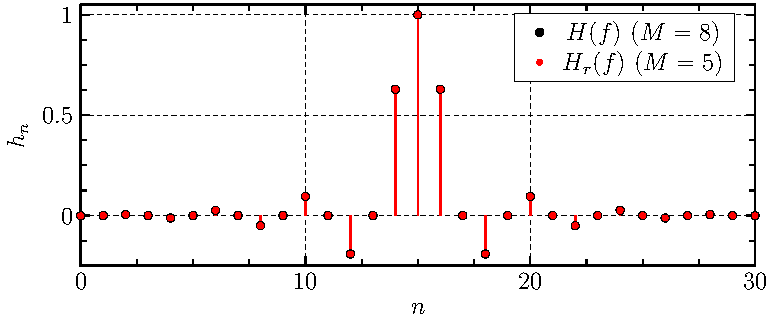
\includegraphics[width=1\linewidth]{imp_resp_hbf32.pdf}
			\label{fig:imp_resp_hbf32}
		\end{subfigure}%
		\begin{subfigure}{.49\textwidth}
			\centering
			\caption{}
			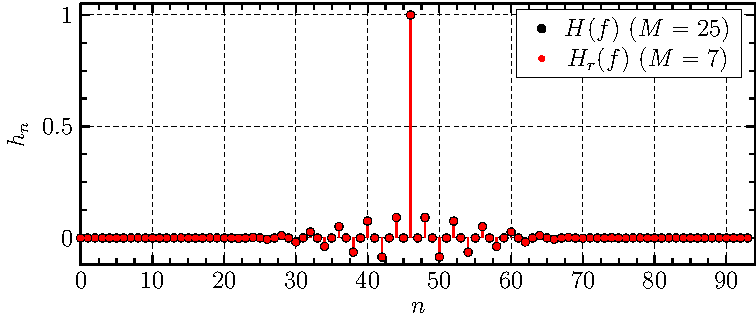
\includegraphics[width=1\linewidth]{imp_resp_hbf96.pdf}
			\label{fig:imp_resp_hbf96}
		\end{subfigure}
		
		\vspace{1cm}  % Расстояние между изображениями, можно настроить
		
		\begin{subfigure}{.49\textwidth}
			\centering
			\caption{}
			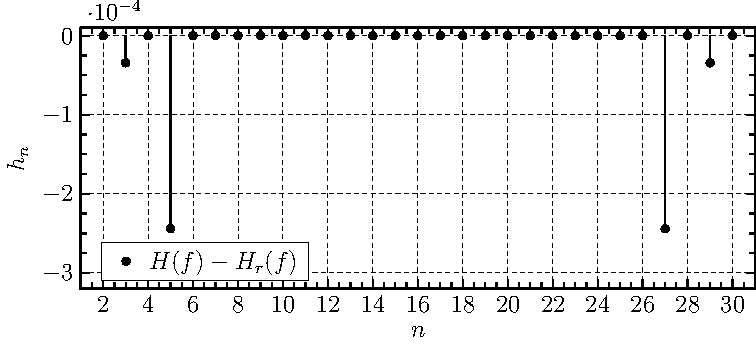
\includegraphics[width=1\linewidth]{imp_resp_hbf32_diff.pdf}
			\label{fig:imp_resp_hbf32_diff}
		\end{subfigure}
		\begin{subfigure}{.5\textwidth}
			\centering
			\caption{}
			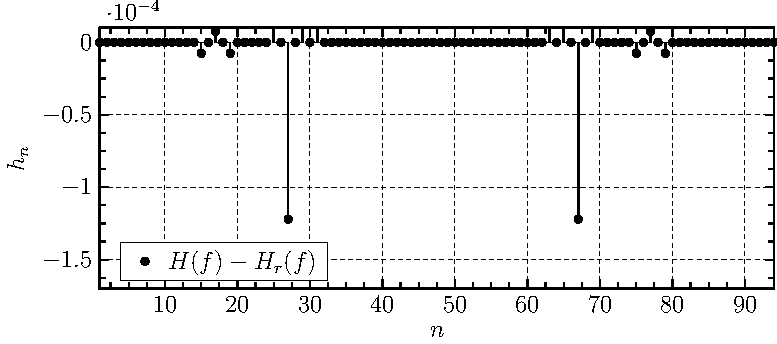
\includegraphics[width=1\linewidth]{imp_resp_hbf94_diff.pdf}
			\label{fig:imp_resp_hbf94_diff}
		\end{subfigure}
%		\caption{(а) --- ИХ изначального и упрощенного ППФ 30 порядка; (б) --- ИХ изначального и упрощенного ППФ 94 порядка}
	\end{figure}
	
	
\end{document}